\section{Related Work}
\subsection{Understanding Deep Neural Networks}
 Deep Learning and DNNs are black-box tools that work well on average on a wide range of tasks. However, due to limited understanding of their behavior, a whole direction of research is dedicated to study and analyze neural networks. There are different lenses to analyze DNNs depending on the purpose of analysis. A famous line of works tries to visualize the network hidden layers by inverting the activations to get a visual image that represents a specific activation  \cite{unn-visual1,unn-visual2,unn-visual3}. Others observe the behavior of these networks under injected noise \cite{unn-robustness-noise1,unn-robustness-noise2,unn-robustness-noise3,unn-robustness-noise4,unn-robustness-noise5,unn-modar}. Sax \etal analyze the deep networks from the lens of information theory and show how the choice of activation layers affect the learning from entropy perspective \cite{info-lense}. Geirhos \etal shows that changing the texture of the object while keeping the borders can hugely deteriorate the recognizability of the object by the DNN \cite{unn-texture}. More closely related to our work is the work of Fawzi \etal, which shows that geometric changes in the image affect the performance of the classifier greatly \cite{unn-robustness-geometry}. They also propose a probabilistic analysis framework to measure the robustness under these nuisance transformations (\eg, perspective and illumination) \cite{unn-robustness-measure}, but they are limited to non-semantic 2D image transformation. 
\subsection{Adversarial Attacks on Deep Neural Networks}
\vspace{-6pt}
\mysection{Pixel-based Adversarial Attacks}
The way that DNNs fail for some noise added to the image motivated the adversarial attacks literature. Szegedy first introduced a formulation of attacking neural networks as an optimization \cite{first-attack}. The method minimizes the perturbation of the image pixels, while still fooling a trained classifier to predict a wrong class label. Several works followed the same approach but with different formulations \cite{fast-sign,projected-gradient,deepfool,carlini}. However, all these methods are limited to pixel perturbations and only fool classifiers, while we consider more general cases of attacks, \eg changes in camera viewpoint to fool a DNN by finding adversarial regions. %withthe perturbation being either in the image or semantic parameters describe the 3D scene from which the image is captured. 
Most of these attacks are white-box attacks, in which the algorithm has access to network gradients. Another direction of adversarial attacks treat the classifiers as a black box, in which the adversary only can quarry points and get a score from the classifier without backpropagating through the DNN \cite{reduc-black,zeroth-order-attack}. We formulate the problem of finding the region as an optimization of the corners of hyper-rectangle in the semantic space in both a black box fashion ( only function evaluations ) as well as the white box formulation which utilizes the gradient of the function.

\mysection{Semantic Adversarial Attacks}
Moving away from pixel perturbation to semantic 3D scene parameters, Zeng \etal \cite{normal-light-attack} generate attacks on deep classifiers by perturbing scene parameters like lighting and surface normals. They show that the most common image space adversarial attacks are not authentic and cannot be realized in real 3D scenes. These semantic parameters are the same parameters studied in the Vision as Inverse Graphics paradigm \cite{old-vision1,old-vision2}. A completely different approach of VIG is to make the graphics operations differentiable from the beginning, which allows for an easy inverting by taking the gradient of the image to the parameters input directly. The most notable work in differentiable rendering is the Neural Mesh renderer (NMR) by Kato \etal \cite{vig-nmr}. NMR approximates the non differentiable rasterization by a differentiable counterpart, allowing the full rendering pipeline to be differentiable and  implementing the technique in Pytorch \cite{paszke2017pytorch}, which lead to broad adoption. We use NMR as our primary rendering method of meshes since we can obtain the gradient of the composite function of the network and the Renderer to the semantic parameters, which is necessary for our Algorithm \ref{alg: white}. Recently Hamdi \etal proposes generic adversarial attacks that incorporate semantic and pixel attacks, in which they define the adversarial attack as sampling from some latent distribution, and they learn a GAN on filtered semantic samples \cite{sada}. However, their work used sampling-based approach to learn these adversarial regions, which does not scale with the dimensionality of the problem.
% When adversarial attacks are studied, two metrics are mainly used to evaluate the  attack: the fooling rate (success rate) and the perceptuality. The first computes the percentage of examples the agent (usually a classifier) actually fooled, while the latter measures the amount of perturbation (usually change in image pixel values).
%  \subsection{Vision as Inverse Graphics (VIG)}
% % \subsection{Vision as Inverse Graphics (VIG)}
% % The paradigm in computer vision of trying to figure out the semantic 3D parameters that generated the image( known as inverse graphics) is an old quest \cite{old-vision1,old-vision2}. The problem is ill-posed and many work around and priors are usually. for more recent works , [] \cite{vig-reinforce} uses REINFORCE to bypass non-differentiability of the OpenGL \cite{opengl} rendering functions and obtain latent representation of 3DMnist. \cite{vig-render-net} proposes architecture of CNN to learn rendering function directly , while \cite{vig-cinvg} learns a rendering function by an auto-encoder that utilizes Auto-Encoding variational Bayes trick \cite{variational-bays} , which allows to invert 3D faces from the rendered images and manipulate them accordingly. \cite{vig-inverse-render-net} learns the inverting function of estimating normals, albidos, and illumination of the scene by multitask learning and utilizing extra information of the normals pre-calculated with Multi View Stereo that is trained on same scene from multiple views. They use a complex spherical harmonics illumination model and try to estimate its parameters during the de-rendering operation. The work of Wu J. \etal \cite{vig-nsd} learns a de-rendering function to predict an XML describing the rendered images from their own proposed 3D Minecraft dataset.  A completely different approach of VIG is to make the graphics operations differentiable from the beginning , which allows for easy inverting by taking the gradient of the image to the parameters input directly. The first work to address this approach is the work of [] which divide the rendering to lighting , vertices , camera and use chain rule to derive the gradient \cite{vig-open-dr}. This approach is used by \cite{vig-one-image} with object detection to predict the latent variables of the object and of the scene for some synthetic and real images of their own. The most notable work in differentiable rendering is the Neural Mesh renderer (NMR) by Kato \etal \cite{vig-nmr} , which approximate the non differentiable rasterization by a differentiable counterpart , allowing the full rendering pipeline to be differentiable and  implementing the technique in Pytorch \cite{paszke2017pytorch}, which lead to wide adoption. [] uses NMR to construct a mesh of some class category without 3D supervision \cite{vig-shape-category}. \cite{vig-scene-manuplation} performs Scene manipulation and 3D-aware image editing by utilizing NMR with other DNNs on some loss.   
\subsection{Optimizing Integral Bounds}
\mysection{Naive Approach} 
To develop an algorithm for robust region finding, we adopt an idea of weekly supervised activity detection in videos by Shou \etal \cite{ioc}. The idea works on maximizing the inner average while minimizing the outer average of the function in the region and optimizing the bounds to achieve the objective. This is achieved because optimizing the bounds to maximize the area exclusively can lead to diverging the bounds to $-\infty,\infty$. To solve the issue of diverging bounds, the following naive formulation is simply regularizing the loss by penalty of the norm of the region size. The expressions for the loss of n=1 dimension is $L = -\text{Area}_{\text{in}} + \frac{\lambda}{2} \left| b-a\right|_{2}^{2} = \int_{a}^{b} f(u)du ~+ \frac{\lambda}{2} \left| b-a\right|_{2}^{2}$, where $f: \mathbb{R}^{1} \rightarrow (0,1)$ is the function of interest and $a,b$ are the left and right bound respectively and $\lambda$ is a hyperparameter. The update directions to minimize the loss are $\pd{L}{a} = f(a) - \lambda (b-a)~,~\pd{L}{b} = - f(b) + \lambda (b-a)$. The regularizer will prevent the region to grow to $\infty$ and the best bounds will be found if loss is minimized with gradient descent or any similar approach.
% \begin{equation}
% \begin{aligned} 
% L = -\text{Area}_{\text{in}} + \frac{\lambda}{2} \left| b-a\right|_{2}^{2}
% \label{eq:loss-naive}
% \end{aligned}
% \end{equation}
% using Libeniz rule as in Lemma \ref{thm:integral}, we get the following update steps for the objective L :
% \begin{equation}
% \begin{aligned} 
% \pd{L}{a} =& f(a) - \lambda (b-a)\\
% \pd{L}{b} =& - f(b) + \lambda (b-a)
% \label{eq:update-ioc-1}
% \end{aligned}
% \end{equation}
% where $\lambda$ is regularizing the boundaries not to extend too much in the case the function evaluation wa positive all the time.
To extend the naive approach to n-dimensions, we will face an another integral in the update direction (hard to compute). Therefore, we deploy the following trapezoid approximation for the integral.

\mysection{Trapezoidal Approximation}
The trapezoidal approximation of definite integrals is a first-order approximation from Newton-Cortes formulas for numerical integration \cite{numerical}. The rule states that $\int_{a}^{b}f(u)du \approx (b-a)\frac{f(a)+f(b)}{2}$.
% \begin{equation}
% \begin{aligned} 
% \int_{a}^{b}f(u)du \approx (b-a)\frac{f(a)+f(b)}{2}
% \label{eq:trapezoidal-integration}
% \end{aligned}
% \end{equation}
An asymptotic error estimate is given by $-\frac { ( b - a ) ^ { 2 } } { 48 } \left[ f ^ { \prime } ( b ) - f ^ { \prime } ( a ) \right] + \mathcal{O} \left( \frac{1}{8} \right)$. So as long the derivatives are bounded by some lipschitz constant $\mathbb{L}$, then the error becomes bounded by the following $|\text{error}| \leq \mathbb{L}( b - a ) ^ { 2 }  $. 
% The regularized loss of interest in \eqLabel{\ref{eq:loss-naive}} becomes 
% $ L = -\text{Area}_{\text{in}} + \lambda \left| b-a\right|_{2}^{2} \approx -(b-a)\frac{f(a)+f(b)}{2} + \lambda \left| b-a\right|_{2}^{2}  $


% \begin{figure*}[t]
% \tabcolsep=0.01cm
%   \begin{tabular}{c|c}
%      Robust regions Growing & dfg edg & df ee &gr e  \\ 
% 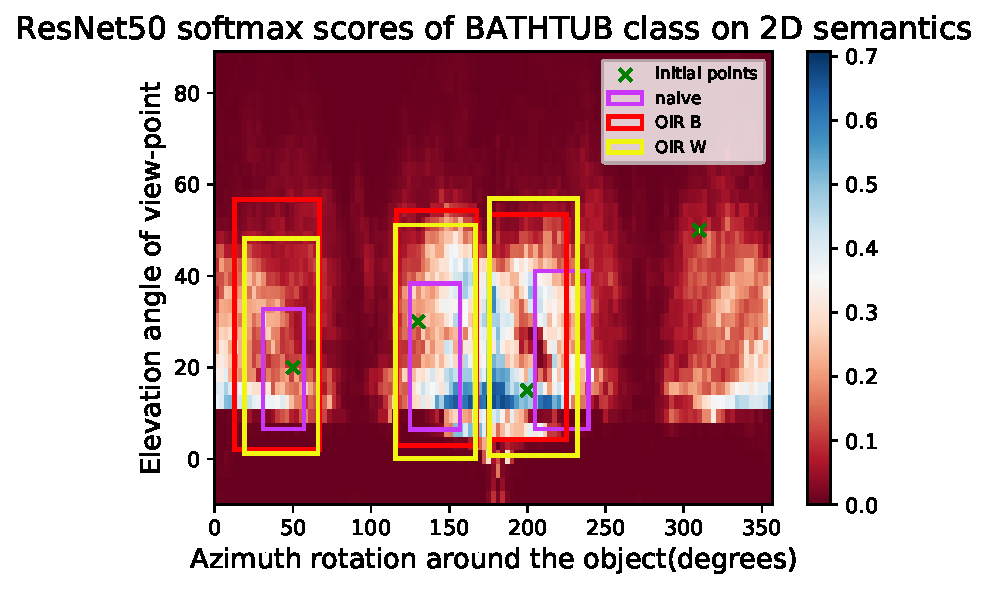
\includegraphics[trim={0.2cm 0.2cm 0.2cm 0.2cm},clip, width = 9cm]{images/pipeline/ResNet50_bathtub_3_regions.pdf} &
%  \\
% 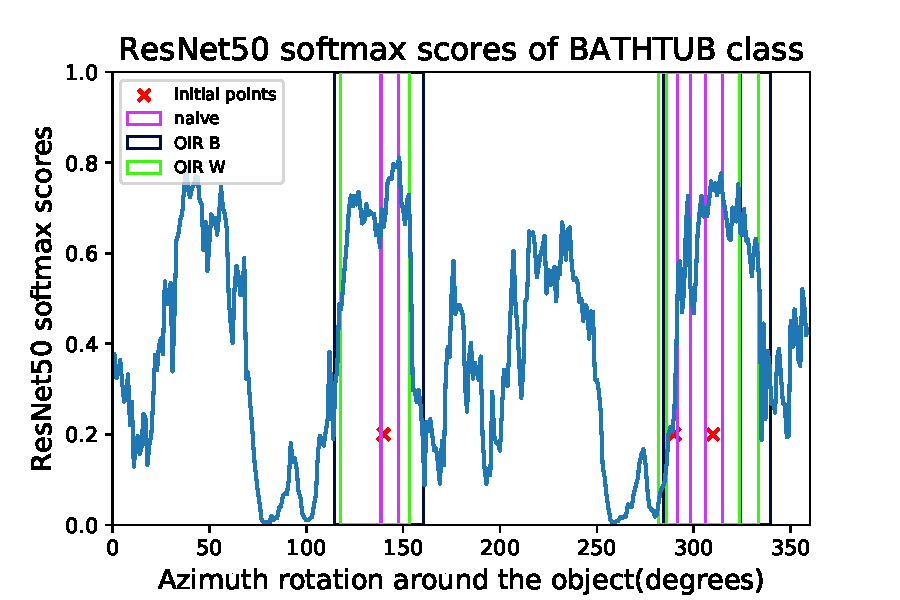
\includegraphics[trim={0.2cm 0.2cm 0.2cm 0.2cm},clip, width = 9cm]{images/pipeline/1D_bathtub_regions.pdf} & 

% \end{tabular}
%   \caption{\small \textbf{Semantic Robustness of Deep Networks}.  the points are [np.array([130,30]),np.array([200,15]),np.array([310,50])] , }
%   \vspace{-8pt}
%   \label{fig:pipeline}
% \end{figure*}


% \begin{figure}[htp]
%     \centering
%     \begin{subfigure}[b]{0.4\textwidth}
%         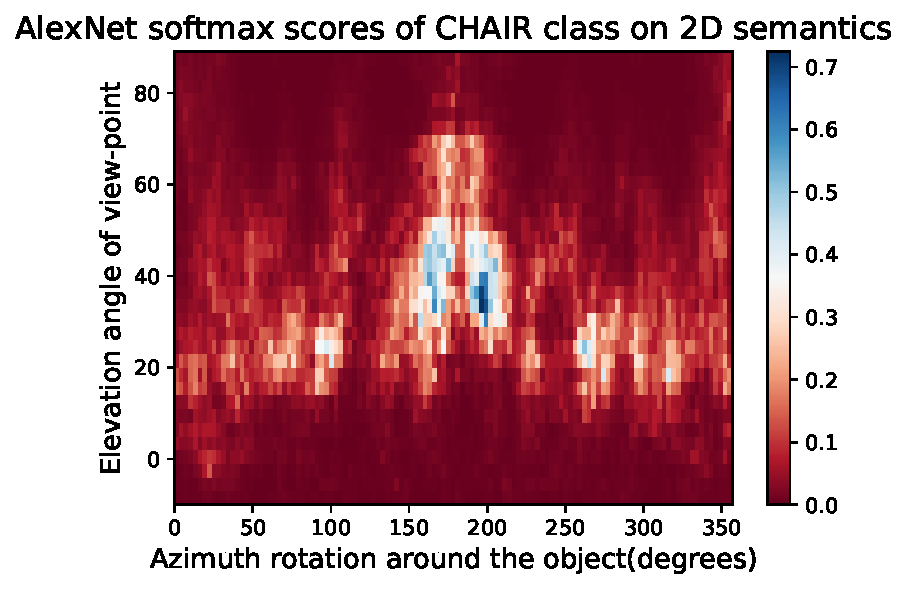
\includegraphics[width=\linewidth]{images/pipeline/AlexNet_chair_7.pdf}
%         \caption{Contact angle with various pseudo dosages}
%         \label{fig:2µm_lines_CA_graph}
%     \end{subfigure}
% \hfil
%     \begin{subfigure}[b]{0.4\textwidth}
%         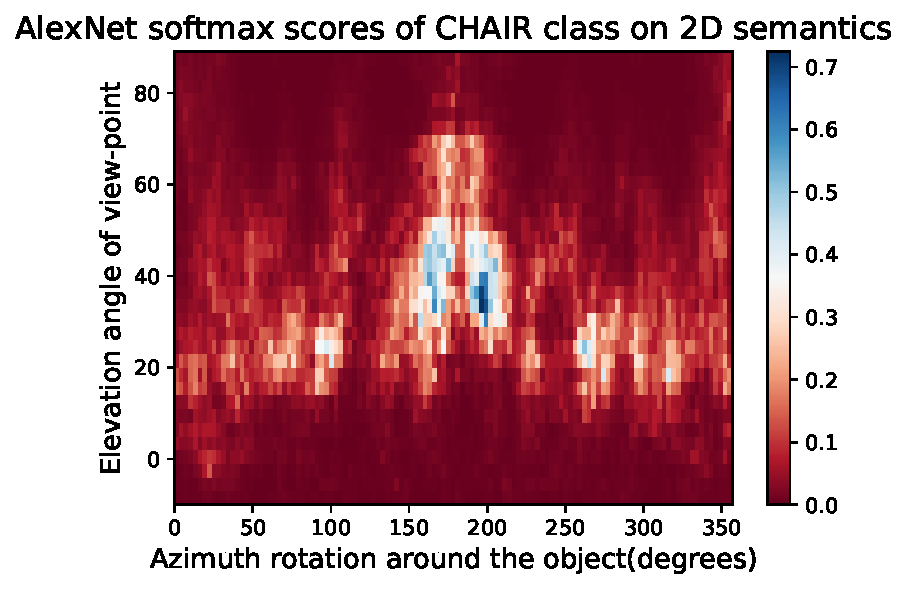
\includegraphics[width=\linewidth]{images/pipeline/AlexNet_chair_7.pdf}
%         \caption{Contact angle with various pseudo dosages}
%         \label{fig:2µm_lines_CAH_graph}
%     \end{subfigure}

%     \begin{subfigure}[b]{0.4\textwidth}
%         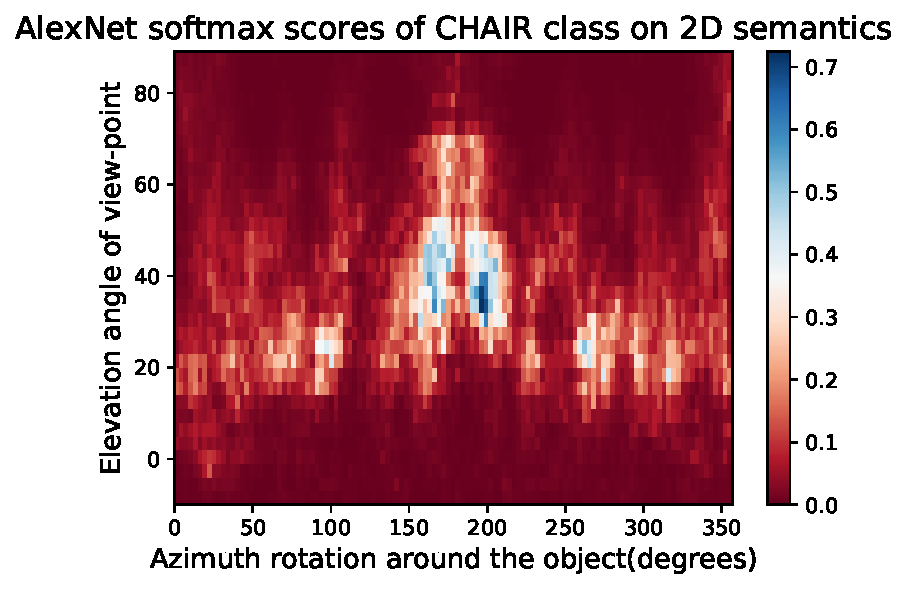
\includegraphics[width=\linewidth]{images/pipeline/AlexNet_chair_7.pdf}
%         \caption{Contact angle with various pseudo dosages}
%         \label{fig:2µm_lines_CA_graph}
%     \end{subfigure}
% \hfil
%     \begin{subfigure}[b]{0.4\textwidth}
%         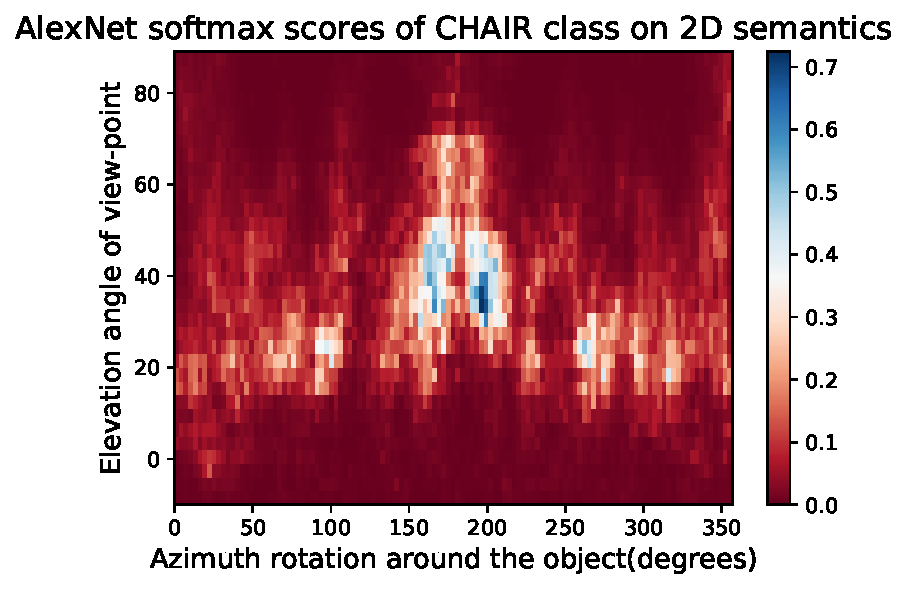
\includegraphics[width=\linewidth]{images/pipeline/AlexNet_chair_7.pdf}
%         \caption{Contact angle with various pseudo dosages}
%         \label{fig:2µm_lines_CAH_graph}
%     \end{subfigure}

%     \begin{subfigure}[b]{0.4\textwidth}
%         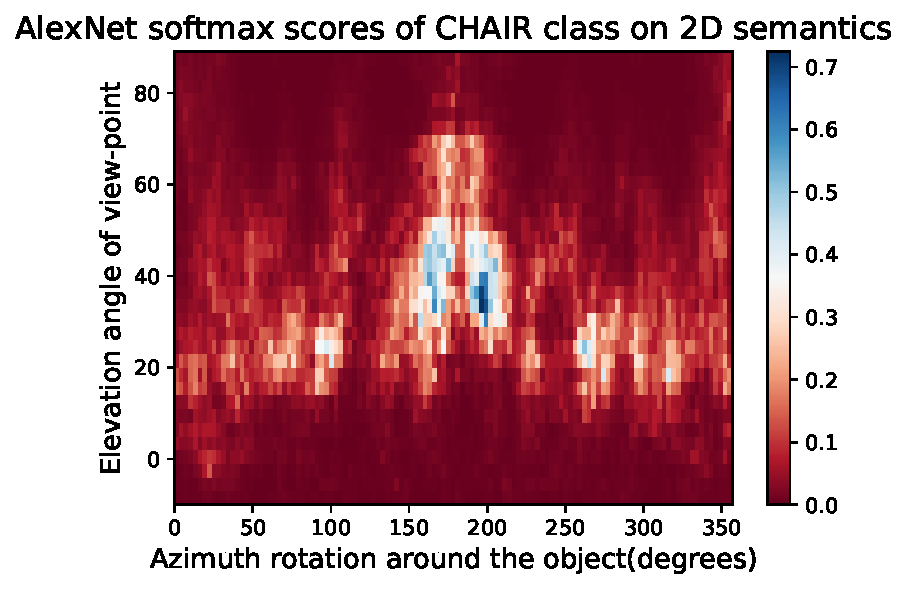
\includegraphics[width=\linewidth]{images/pipeline/AlexNet_chair_7.pdf}
%         \caption{Contact angle with various pseudo dosages}
%         \label{fig:2µm_lines_CA_graph}
%     \end{subfigure}
% \hfil
%     \begin{subfigure}[b]{0.4\textwidth}
%         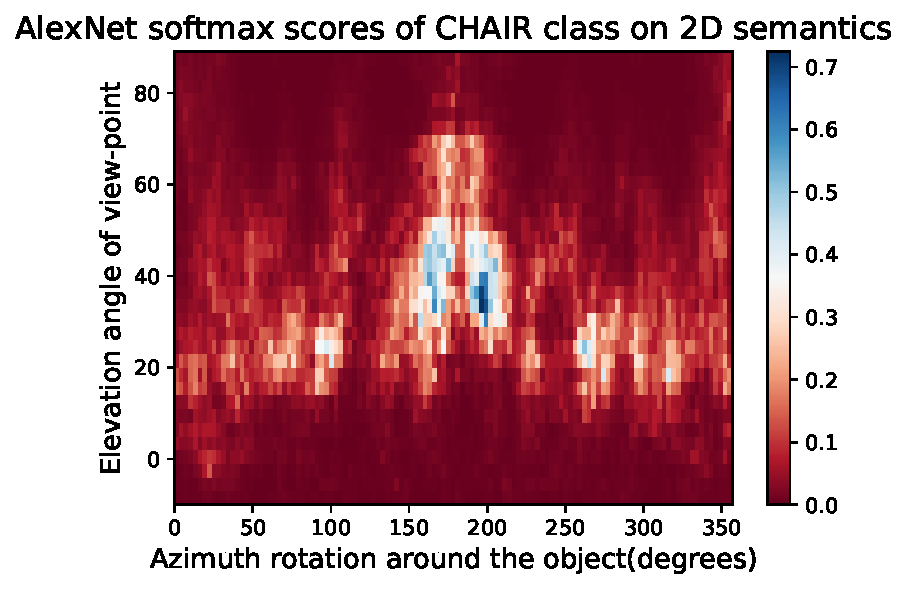
\includegraphics[width=\linewidth]{images/pipeline/AlexNet_chair_7.pdf}
%         \caption{Contact angle with various pseudo dosages}
%         \label{fig:2µm_lines_CAH_graph}
%     \end{subfigure}

%     \begin{subfigure}[b]{0.4\textwidth}
%         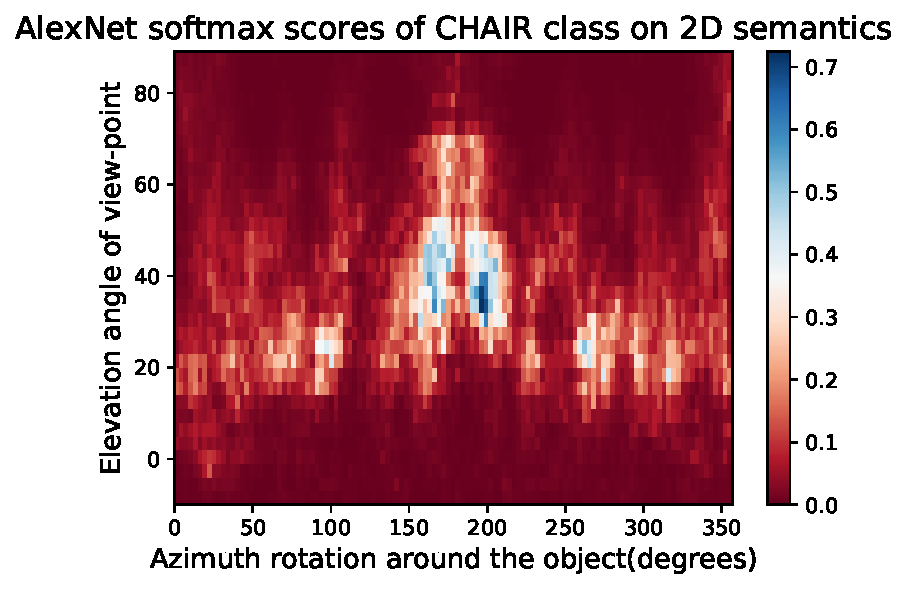
\includegraphics[width=\linewidth]{images/pipeline/AlexNet_chair_7.pdf}
%         \caption{Contact angle with various pseudo dosages}
%         \label{fig:2µm_lines_CA_graph}
%     \end{subfigure}
% \hfil
%     \begin{subfigure}[b]{0.4\textwidth}
%         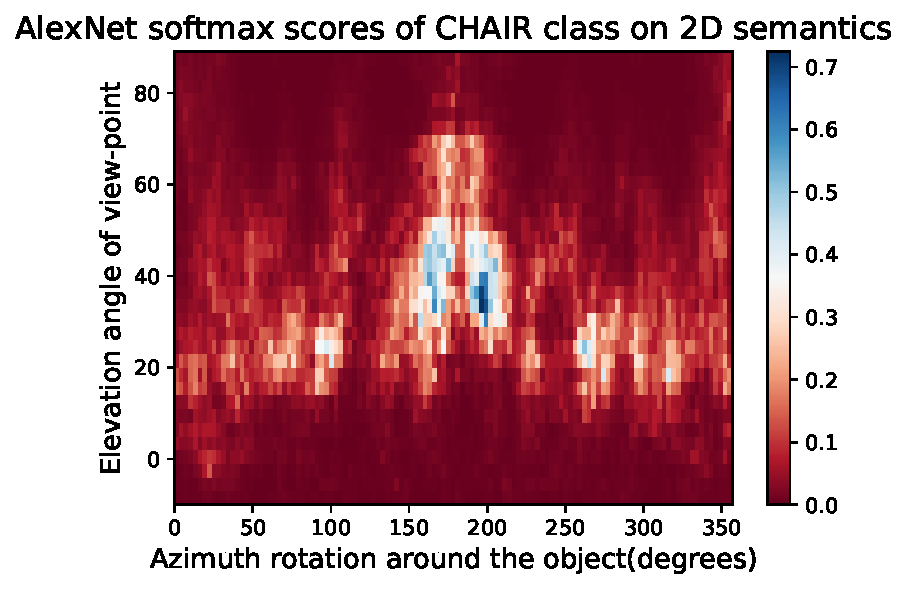
\includegraphics[width=\linewidth]{images/pipeline/AlexNet_chair_7.pdf}
%         \caption{Contact angle with various pseudo dosages}
%         \label{fig:2µm_lines_CAH_graph}
%     \end{subfigure}
%     \caption{Contact angles on 2 $\mu$m Lines}\label{fig:2µm_lines_CA_graphs}
% \end{figure}



% \begin{figure*}[t]
% \tabcolsep=0.01cm
%   \begin{tabular}{c|c}
%      Robust regions Growing & dfg edg & df ee &gr e  \\ 
% 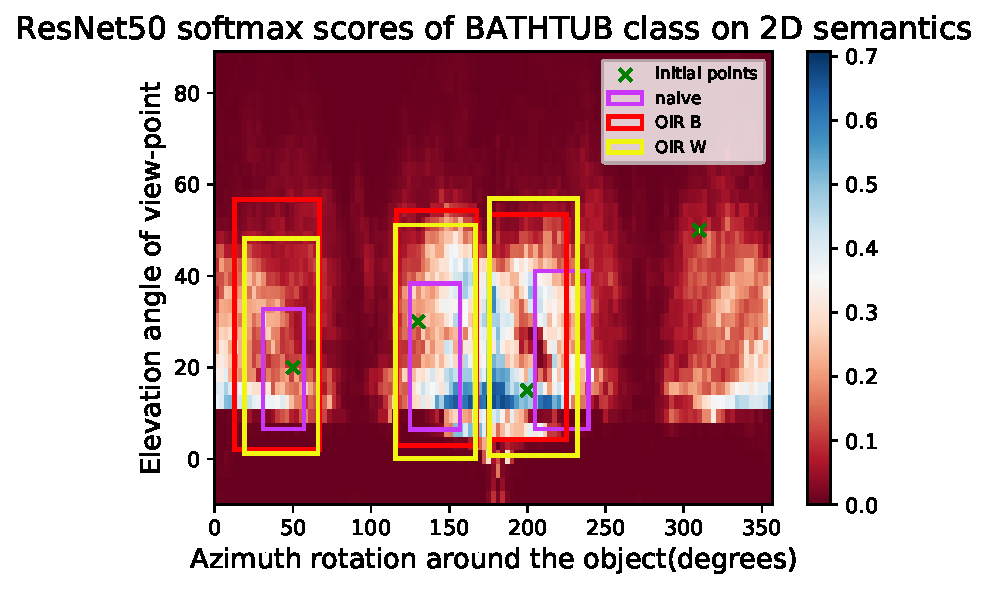
\includegraphics[trim={0.2cm 0.2cm 0.2cm 0.2cm},clip, width = 9cm]{images/pipeline/ResNet50_bathtub_3_regions.pdf} &
%  \\
% 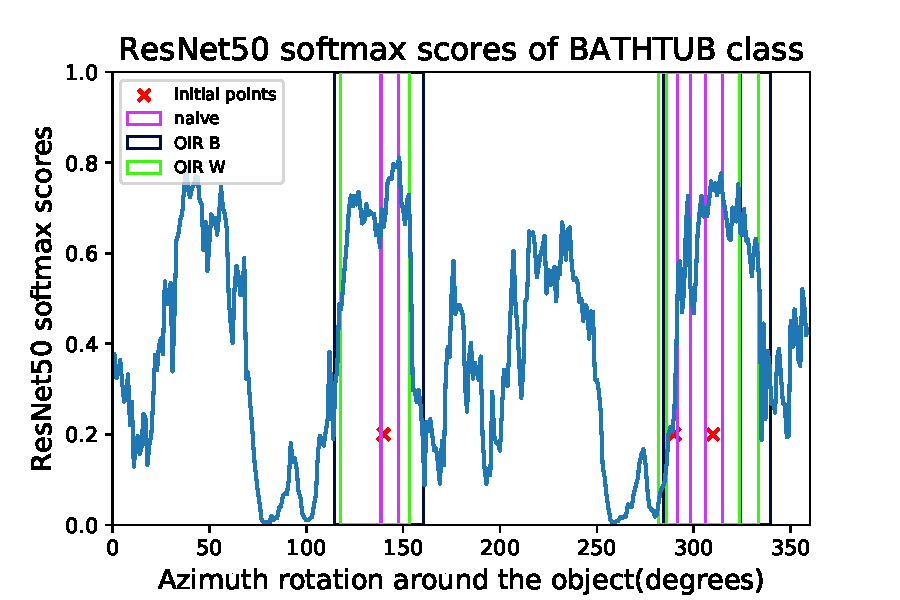
\includegraphics[trim={0.2cm 0.2cm 0.2cm 0.2cm},clip, width = 9cm]{images/pipeline/1D_bathtub_regions.pdf} & 

% \end{tabular}
%   \caption{\small \textbf{Semantic Robustness of Deep Networks}.  the points are [np.array([130,30]),np.array([200,15]),np.array([310,50])] , }
%   \vspace{-8pt}
%   \label{fig:pipeline}
% \end{figure*}

\begin{figure*}[t]
\centering
    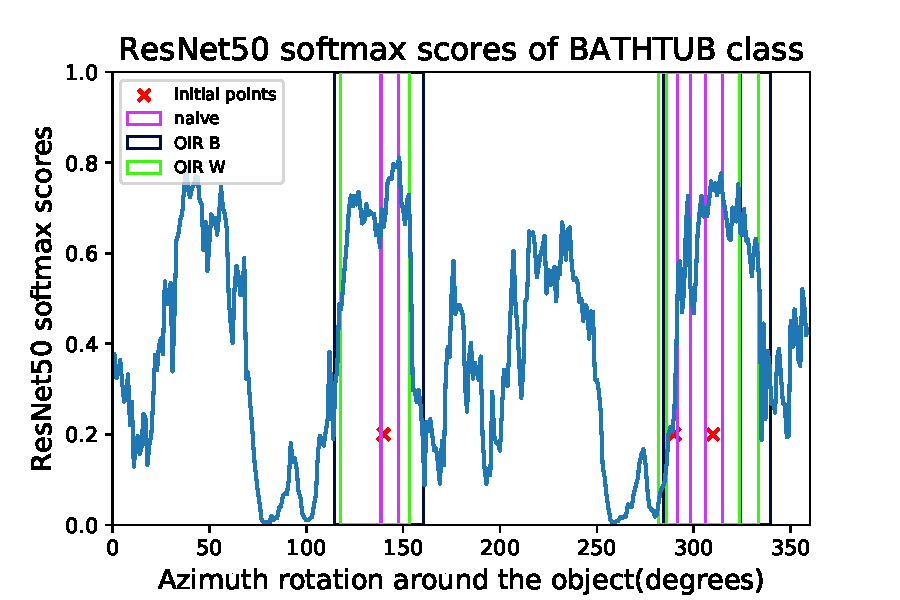
\includegraphics[width=.49\linewidth]{images/pipeline/1D_bathtub_regions.pdf}
  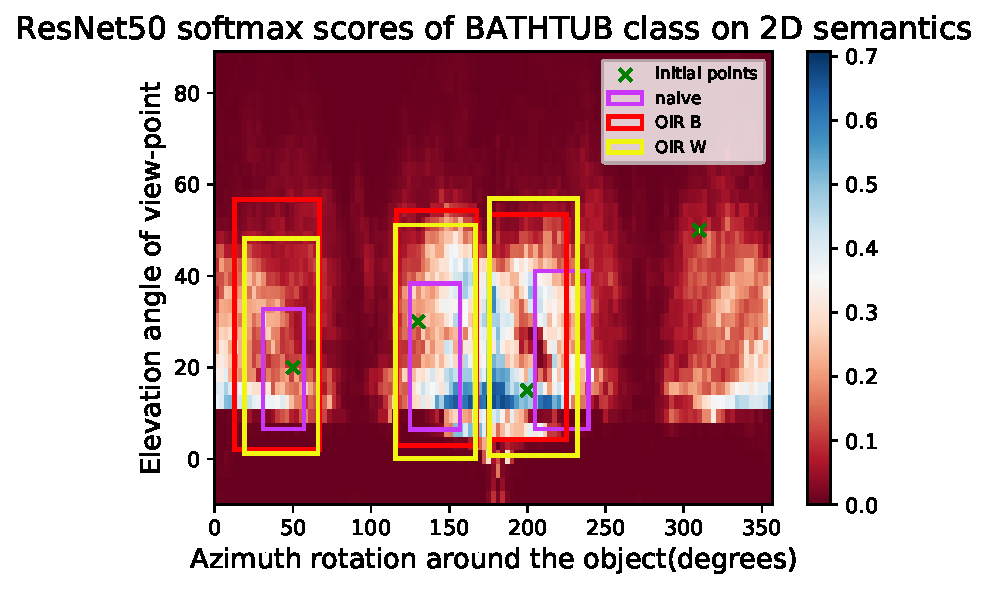
\includegraphics[width=.50\linewidth]{images/pipeline/ResNet50_bathtub_3_regions.pdf}
\vspace{-9pt}
\caption{ \small \textbf{Semantic Robust Region Finding}: finding robust regions of semantic parameters for Rsnet50 \cite{resnet} in a bathtub object by the three bottom-up formulations (naive , OIR\_W , OIR\_B). (\textit{left}): 1D case (azimuth angle of camera) with three initial points points. (\textit{right}): 2D case (azimuth angle and elevation angle of camera) with four initial points. We note that the naive approach usually predicts smaller regions, while the OIR formulations finds more comprehensive regions.}
\label{fig:operator}
\vspace{-9pt}
\end{figure*}


\begin{figure*}[t]
\centering
\tabcolsep=0.08cm
  \begin{tabular}{c|c|c|c}
  \textbf{AlexNet}\cite{AlexNet} & \textbf{VGG}\cite{vgg} & \textbf{Resnet50}\cite{resnet} & \textbf{InceptionV3}\cite{inception} \\
  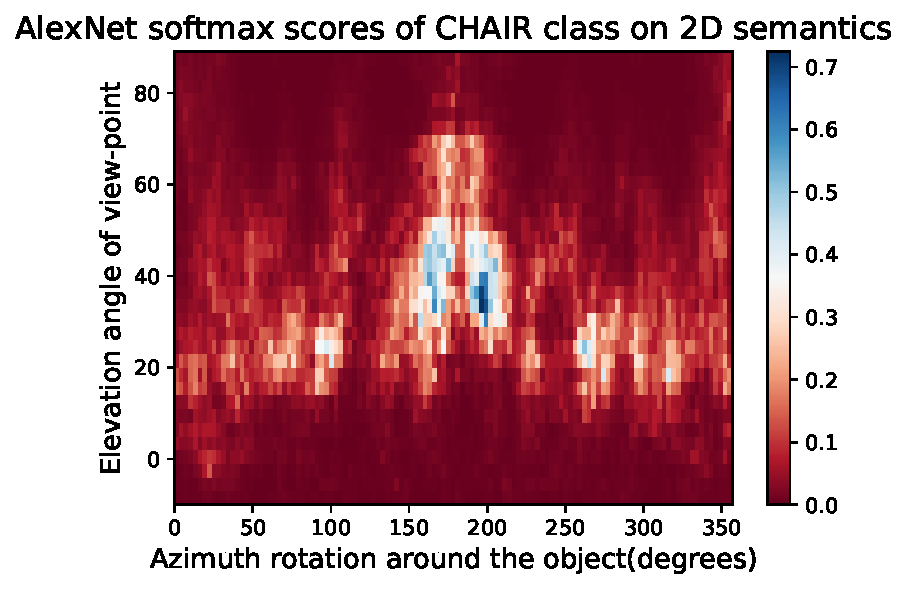
\includegraphics[trim={3cm 1.4cm 2.8cm 1.2cm},clip, width=.24\linewidth]{images/pipeline/AlexNet_chair_7.pdf}&
  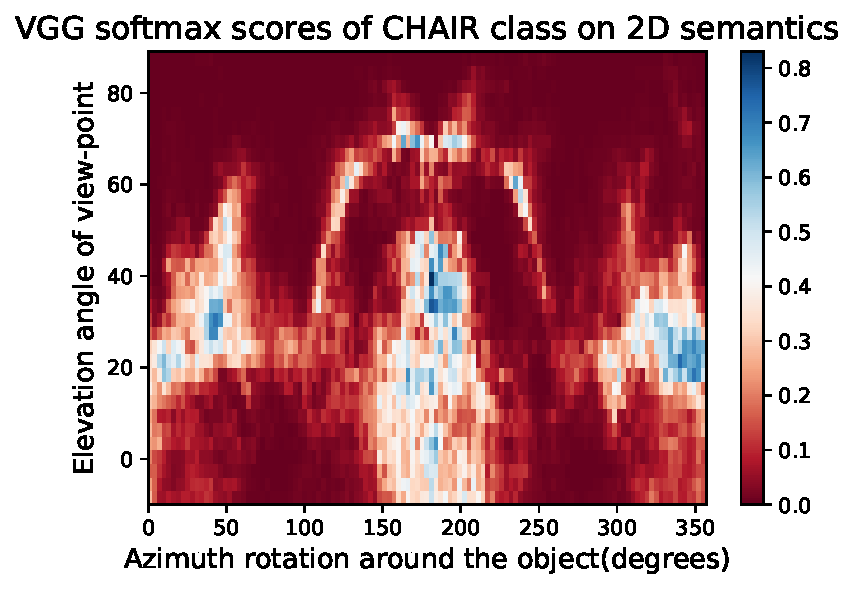
\includegraphics[trim={3cm 1.8cm 2.8cm 1.2cm},clip, width=.23\linewidth]{images/pipeline/VGG_chair_7.pdf}&
  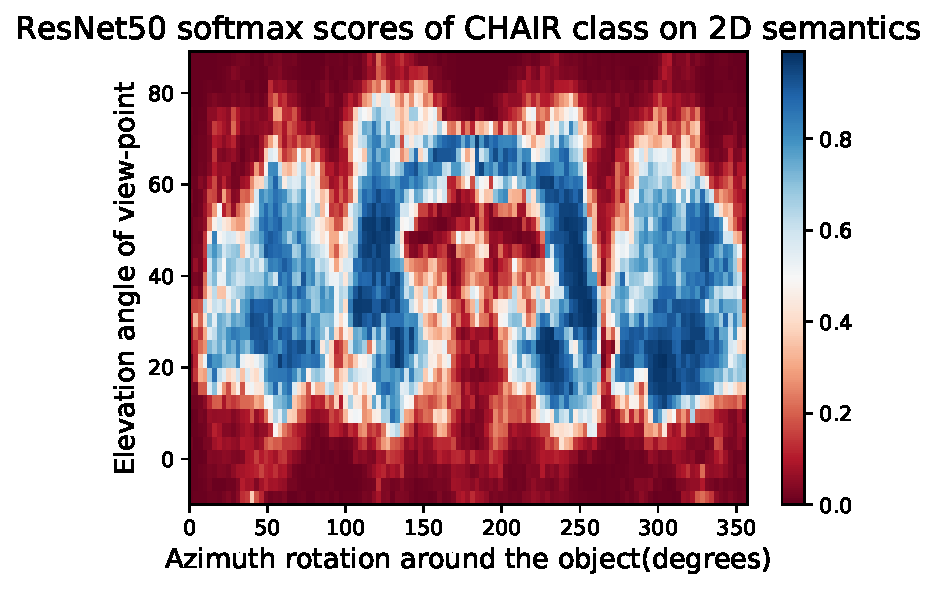
\includegraphics[trim={3.2cm 1.4cm 2.8cm 1.4cm},clip, width=.257\linewidth]{images/pipeline/ResNet50_chair_7.pdf}&
  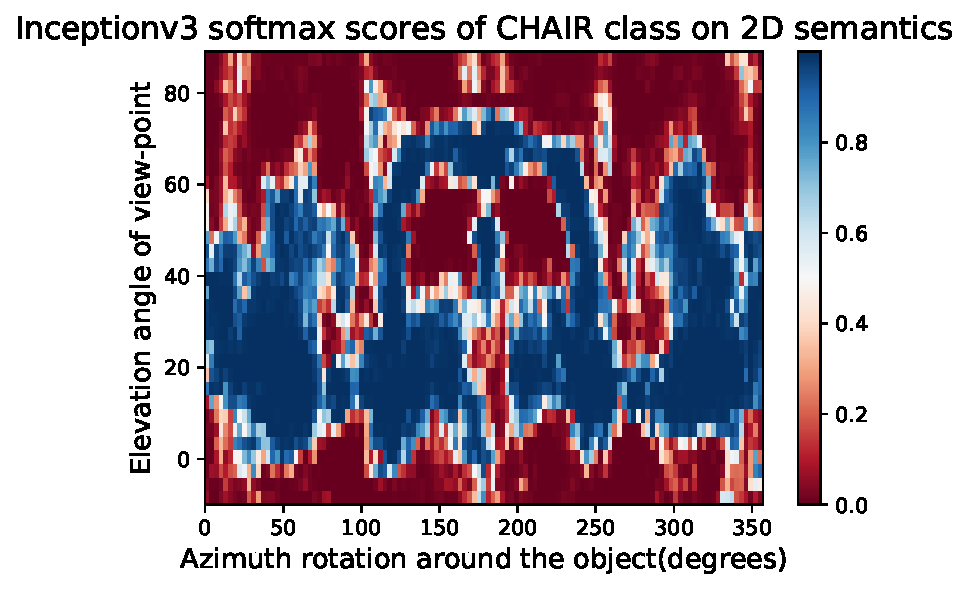
\includegraphics[trim={3.5cm 1.4cm 3cm 1.4cm},clip, width=.259\linewidth]{images/pipeline/Inceptionv3_chair_7.pdf} \\ \hline
  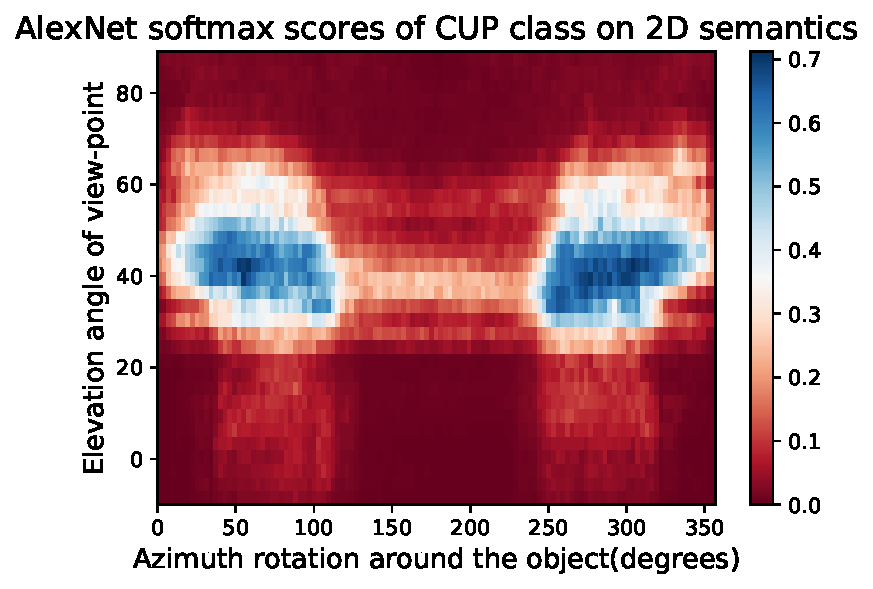
\includegraphics[trim={3cm 1.4cm 2.8cm 1.2cm},clip, width=.24\linewidth]{images/pipeline/AlexNet_cup_4.pdf}&
  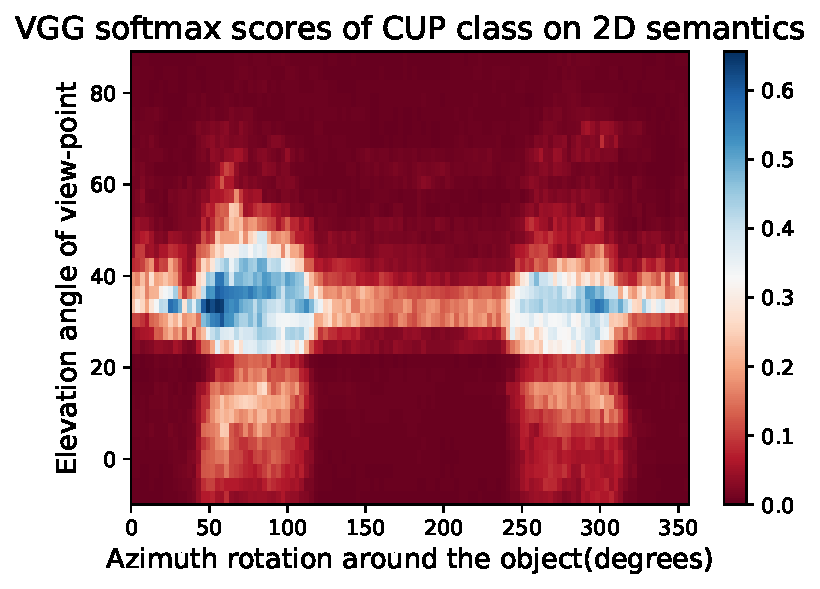
\includegraphics[trim={3cm 1.85cm 2.8cm 1.2cm},clip, width=.23\linewidth]{images/pipeline/VGG_cup_4.pdf}&
  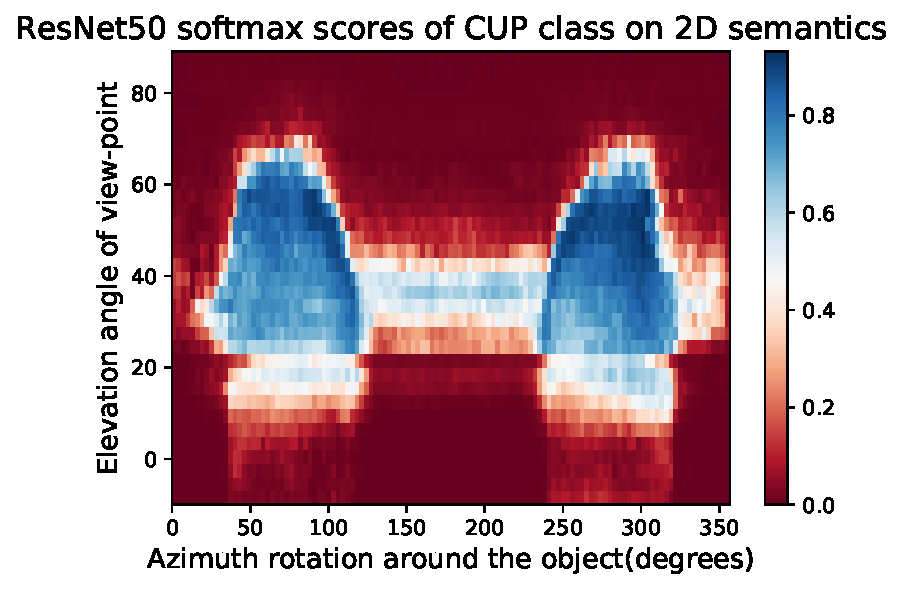
\includegraphics[trim={3cm 1.4cm 2.8cm 1.2cm},clip, width=.25\linewidth]{images/pipeline/ResNet50_cup_4.pdf} &
  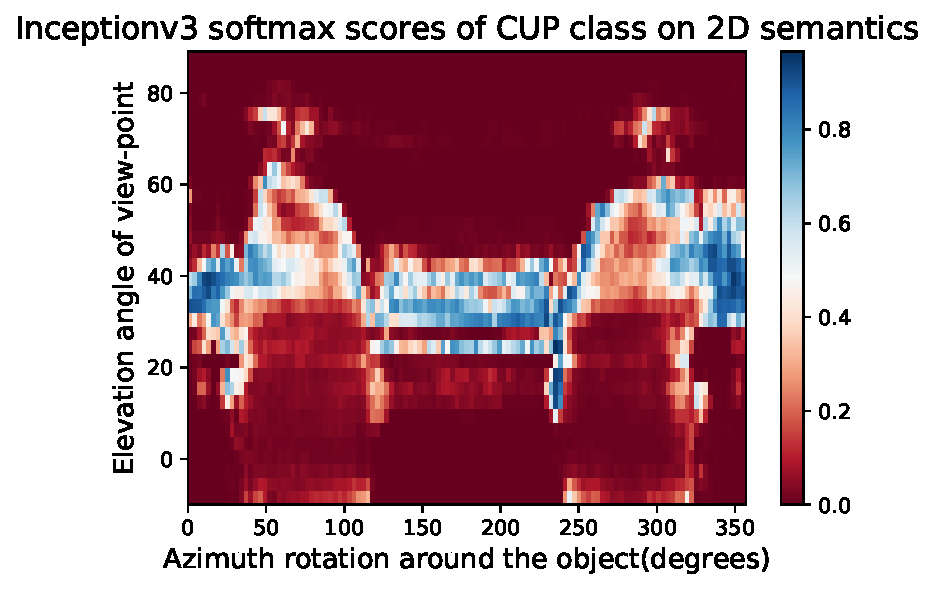
\includegraphics[trim={3.2cm 1.4cm 2.8cm 1.2cm},clip, width=.259\linewidth]{images/pipeline/Inceptionv3_cup_4.pdf} \\
   \end{tabular}
\vspace{-9pt}
\caption{ \small \textbf{Network Semantic Maps}: plotting the 2D semantic maps (as in \figLabel{\ref{fig:operator} \textit{right}}) of four different networks on two shapes of a chair class (\textit{top}) and cup class (\textit{bottom}).% From left to right the networks are: AlexNet\cite{AlexNet},VGG\cite{vgg},Resnet50\cite{resnet},and InceptionV3\cite{inception}.
 We note that InceptionV3 is very confident about its decision , but the cost is that it creates semantic ``traps" where a sharp fall of performance happens in the middle of a robust region. This behaviour is more apparent for complex shapes (\eg the chair in \textit{top} row)}
\label{fig:NMS}
\vspace{-9pt}
\end{figure*}
